\documentclass{article}
\usepackage[utf8]{inputenc}
\usepackage[turkish]{babel}
\usepackage{textcomp}
\usepackage{amsmath}
\usepackage{graphicx}
\usepackage{kvsetkeys}
\let\setkeys\kvsetkeys
\graphicspath{{./images/}}

\title{Ödev 4 Rapor}
\author{Oğuz Kahraman - 18501051}

\begin{document}
	\maketitle

	\section{Başlangıç noktası}
	Başlangıç noktası 1000 parçacık için 0 seçildiğinden aşağıdaki görüntü oluşur.
	\begin{center}
		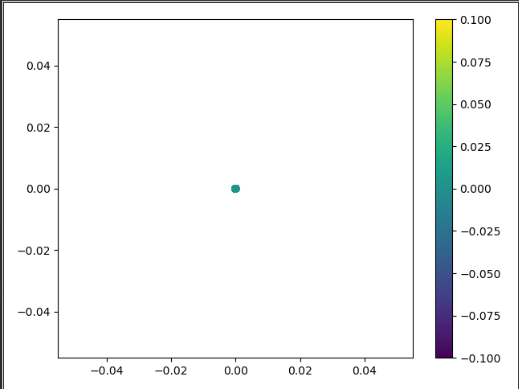
\includegraphics[scale=0.8]{startpoint}
	\end{center}

	\section{Parçacık Üretiimi ve Değerlerin Seçimi}
	Burada hata değerleri olan a1, a2, a3 ve a4 değeleri robotların dağılımında önemli etken çünkü değer büyüdükçe hata ihtimali nüyüyor demektir. O nedenle ne kadar küçük seçersek robotlar o kadar bir arada kalıyor. 
	İlk olarak değerler aşağıdaki gibi seçilince sonuç grafiklerini ekledim.\\
	a1=a2=a3=a4=0.01
		\begin{center}
		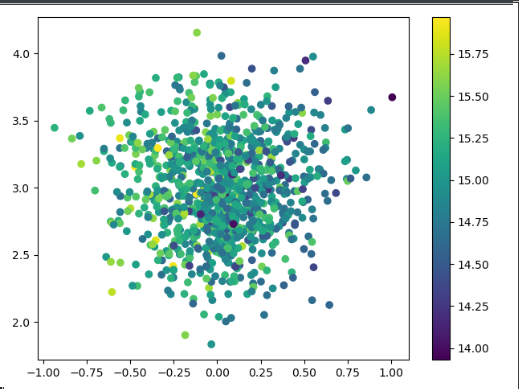
\includegraphics[scale=0.4]{step1}
		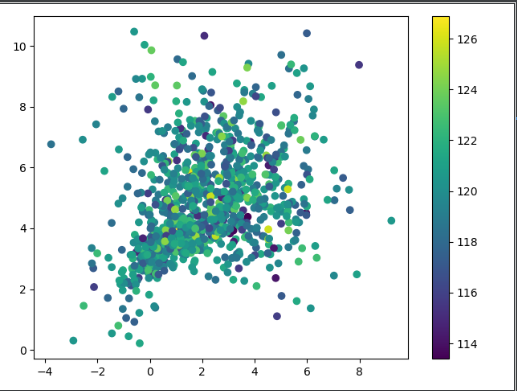
\includegraphics[scale=0.4]{step2}
		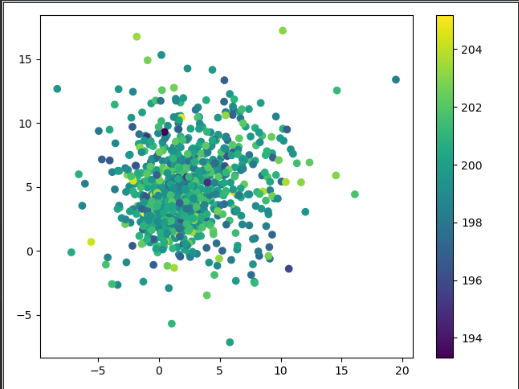
\includegraphics[scale=0.4]{step3}
		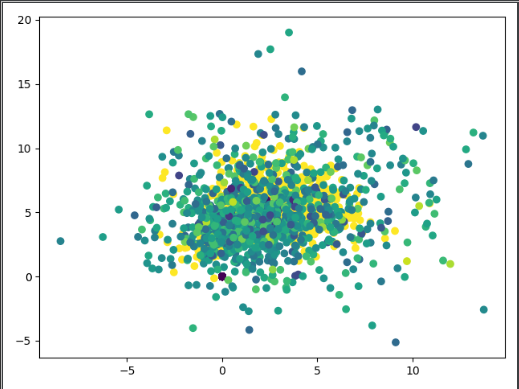
\includegraphics[scale=0.4]{step3.1}
		
	\end{center}
	İkinci olarak değerler aşağıdaki gibi seçilince sonuç grafiklerini ekledim.\\
	a1=a2=a3=a4=0.001
		\begin{center}
		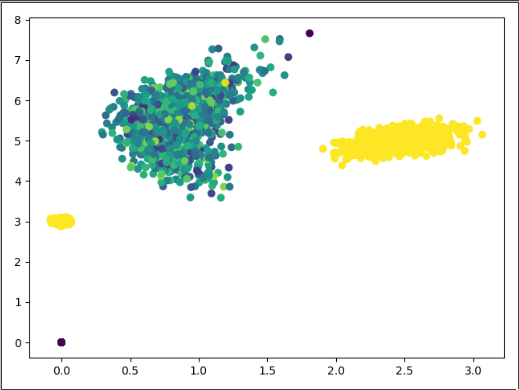
\includegraphics[scale=0.4]{step7}
		
	\end{center}
		Son olarak değerler aşağıdaki gibi seçilince sonuç grafiklerini ekledim.\\
	a1=0.001 a2=0.002 a3=0.003 a4=0.004
		\begin{center}
		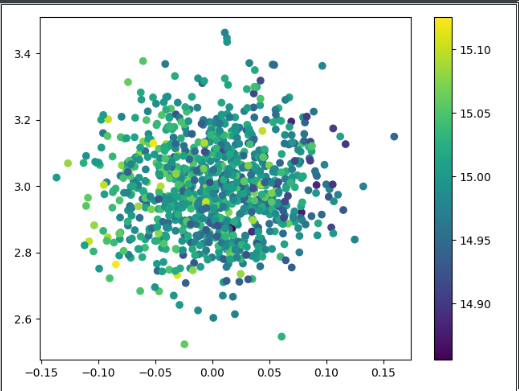
\includegraphics[scale=0.4]{step4}
		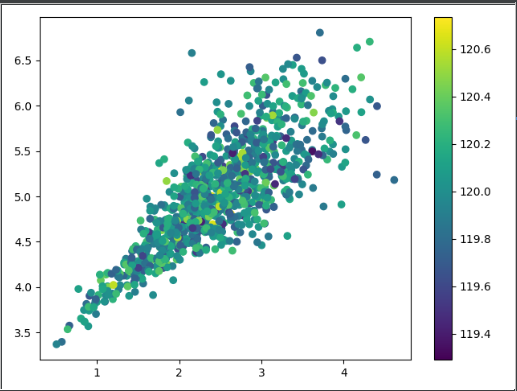
\includegraphics[scale=0.4]{step5}
		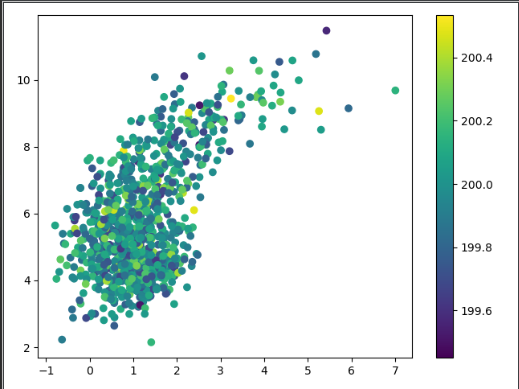
\includegraphics[scale=0.4]{step6}
		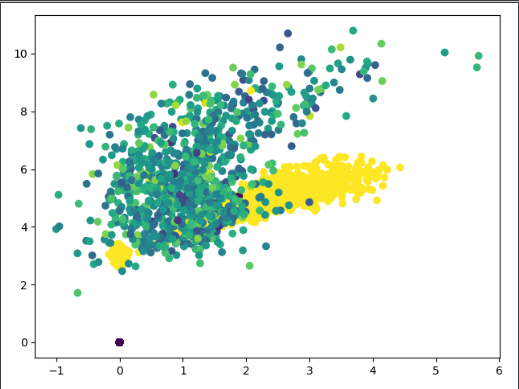
\includegraphics[scale=0.4]{step6.1}
	\end{center}
\section{Sonuç}
Sonuç olarak burada hata değerleri çok kritik. Ne kadar küçük alınırsa robotlar her hareket sonrası o kadar bir arada, ne kadar yüksek alınırsa o kadar karışık olur. Değelerin seçimi de robotların ne kadar dağılacağı konusunda önemli bir yer almaktadır.
\end{document}
